\section{等可能模型}
\label{sec:cprob-equally-likely}

一枚做工均匀的骰子，六个面在形状和重量上没有区别，我们找不到任何理由认为某一面更容易朝上。既然如此，就让六个面分得同样多的可能性，各占$1/6$。“出现偶数点”包含三个面，它的可能性就是$3/6$。把这个想法推广到一般的有限样本空间，就得到用计数定义的概率。

\paragraph{计数比}
可以把概率想成一份总量为$1$的质量，要分配到样本空间的各个点上。等可能就是平均分配：$\Omega$有$\lvert\Omega\rvert$个点，每个点分到$1/\lvert\Omega\rvert$。一个事件的概率，就是落在这个事件区域里的质量总和。点的质量相同，总和就等于点数乘以每点的质量。

\begin{definition}[古典概率]
\label{def:cprob-classical}
设样本空间$\Omega$有限且非空，并假设每个样本点同样可能出现。对每个事件$A\subseteq\Omega$，令
\begin{equation}
 \mathbb{P}(A)=\frac{\lvert A\rvert}{\lvert\Omega\rvert},
 \label{eq:cprob-classical}
\end{equation}
其中$\lvert A\rvert$是$A$的元素个数。称$\mathbb{P}(A)$为事件$A$的概率，称$(\Omega,\mathbb{P})$为\term{古典概率模型}（classical probability model）。
\end{definition}

式~\eqref{eq:cprob-classical}把概率问题完全化成了计数问题：分子数事件里的结果，分母数全部结果，两者都在同一个样本空间里数。每个基本事件的概率都是$1/\lvert\Omega\rvert$，这正是“等可能”的数学表述。

\paragraph{三条基本性质}
这个定义给出的数满足哪些规律？我们希望概率像“占比”一样运算：不会是负数，全体的占比是$1$，两块不重叠的部分合起来，占比相加。下面验证计数比确实具有这三条性质；后面的一切运算规则都从它们推出。

\begin{theorem}[古典概率的基本性质]
\label{thm:cprob-axioms}
在古典概率模型中，对任意事件$A,B$：
\begin{enumerate}
 \item 非负性：
 \begin{equation}
  \mathbb{P}(A)\geq0;
  \label{eq:cprob-nonneg}
 \end{equation}
 \item 归一性：
 \begin{equation}
  \mathbb{P}(\Omega)=1;
  \label{eq:cprob-normalized}
 \end{equation}
 \item 互斥可加性：若$A\cap B=\varnothing$，则
 \begin{equation}
  \mathbb{P}(A\cup B)=\mathbb{P}(A)+\mathbb{P}(B).
  \label{eq:cprob-additive}
 \end{equation}
\end{enumerate}
\end{theorem}

\begin{proof}
元素个数非负，分母$\lvert\Omega\rvert$为正，所以$\mathbb{P}(A)\geq0$。取$A=\Omega$，分子分母相同，比值为$1$。

若$A\cap B=\varnothing$，并集$A\cup B$中的每个元素恰好属于$A$与$B$中的一个，按计数的加法规则
\[
 \lvert A\cup B\rvert=\lvert A\rvert+\lvert B\rvert.
\]
两边同除以$\lvert\Omega\rvert$，就得到式~\eqref{eq:cprob-additive}。
\end{proof}

互斥可加性对有限个两两互斥的事件同样成立。设$A_1,\ldots,A_m$两两互斥，对$m$归纳：$A_1\cup\cdots\cup A_{m-1}$与$A_m$互斥，用一次式~\eqref{eq:cprob-additive}，再用归纳假设，得到
\[
 \mathbb{P}(A_1\cup\cdots\cup A_m)=\mathbb{P}(A_1)+\cdots+\mathbb{P}(A_m).
\]
特别地，任何事件都是它所含基本事件的互斥并，所以$\mathbb{P}(A)$等于$A$中各点概率之和。这与开头“质量总和”的图景一致。

反过来，计数比也是唯一与等可能相容的分配。设某种分配满足三条基本性质，并且每个基本事件的概率都等于同一个数$c$。$\Omega$是它的$\lvert\Omega\rvert$个基本事件的互斥并，由有限可加性与归一性，
\[
 1=\mathbb{P}(\Omega)=\lvert\Omega\rvert\,c,
\]
所以$c=1/\lvert\Omega\rvert$；再对$A$的各点求和，就得到$\mathbb{P}(A)=\lvert A\rvert/\lvert\Omega\rvert$。因此定义~\ref{def:cprob-classical}并没有额外的选择：一旦接受等可能假设和三条性质，概率只能是计数比。

\paragraph{两枚骰子}
掷两枚骰子，把它们看成可区分的第一枚与第二枚，结果记为有序对$(i,j)$，$i,j\in\{1,\ldots,6\}$。样本空间有$36$个点。若每枚骰子都均匀，两次投掷互不干扰，我们就假设这$36$个有序对同样可能。

图~\ref{fig:cprob-dice-grid}把$36$个结果排成方格，格中写的是点数和$i+j$。点数和相同的格子排在同一条斜线上。事件“点数和为$7$”占$6$格，“点数和为$2$”只占$1$格，于是
\[
 \mathbb{P}(\text{点数和为}7)=\frac{6}{36}=\frac16,\qquad
 \mathbb{P}(\text{点数和为}2)=\frac{1}{36}.
\]

\begin{BookInlineFigure}
  \centering
  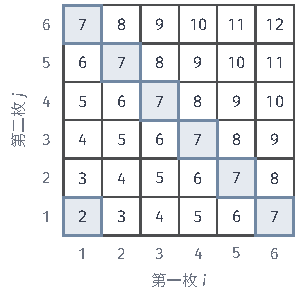
\includegraphics[width=51mm]{figures/07-probability/01-elementary-probability/tikz/cprob-dice-grid/figure.pdf}
  \caption{两枚骰子的$36$个等可能结果。横向是第一枚的点数$i$，纵向是第二枚的点数$j$，格中数字是点数和。浅蓝格子是事件“点数和为$7$”（$6$格）与“点数和为$2$”（$1$格）。}
  \label{fig:cprob-dice-grid}
\end{BookInlineFigure}

点数和从$2$到$12$共$11$种。如果以这$11$个值为样本点，并认为它们同样可能，每个值的概率就都是$1/11$。这与计数结果矛盾：和为$7$的出法有$6$种，和为$2$只有$(1,1)$一种。以点数和为样本点并没有错，错的是对它们使用了等可能假设。

\paragraph{等可能是模型假设}
上面的矛盾说明，式~\eqref{eq:cprob-classical}的前提“每个样本点同样可能”不是从样本空间的写法推出来的，而是对试验所作的假设。它的依据是试验的物理对称性：骰子各面均匀，牌洗得充分，摸球前搅匀且每个球被摸到的机会相同。样本点的名称看起来对称，并不构成这样的依据。

历史上一个有名的错误是这样的：抛两枚硬币，结果分为“两正”“两反”“一正一反”三种，于是认为每种的概率都是$1/3$。按硬币区分先后，等可能的结果是“正正”“正反”“反正”“反反”四种，“一正一反”占了其中两种，所以
\[
 \mathbb{P}(\text{两正})=\frac14,\qquad
 \mathbb{P}(\text{一正一反})=\frac12.
\]
三种结果的名称同样简单，但它们合并的基本结果个数不同，不能平分概率。

哪个模型对，可以用重复试验来检验。把同一试验重复许多次，事件发生的次数除以试验次数称为事件的\term{相对频率}（relative frequency）。图~\ref{fig:cprob-coin-frequency}模拟了$2000$轮抛两枚硬币：随着轮数增加，“两正”的相对频率稳定在$1/4$附近，“一正一反”稳定在$1/2$附近，都远离$1/3$。

\begin{BookInlineFigure}
  \centering
  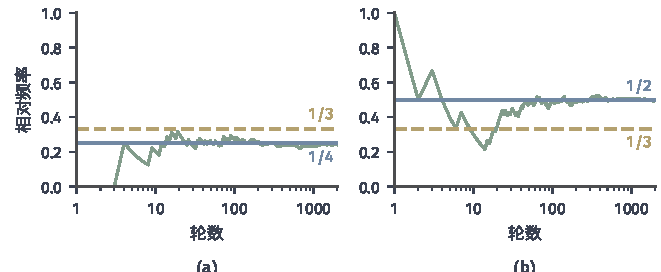
\includegraphics[width=112mm]{figures/07-probability/01-elementary-probability/matplotlib/cprob-coin-frequency/figure.pdf}
  \caption{抛两枚均匀硬币$2000$轮的模拟（随机数种子$3$），横轴为对数坐标。绿线是前若干轮中事件的相对频率，蓝线是四个有序结果等可能时的概率，黄色虚线是错误地认为三种结果等可能时的$1/3$。(a)两正；(b)一正一反。$2000$轮后两个频率分别是$0.2415$和$0.496$。}
  \label{fig:cprob-coin-frequency}
\end{BookInlineFigure}

图~\ref{fig:cprob-dice-sum-frequency}对两枚骰子做了同样的检验。$3600$次模拟中，各点数和的相对频率紧贴计数比$k/36$，其中$k$是该点数和所占的格子数；它们与$1/11$的水平线则明显不符。

\begin{BookInlineFigure}
  \centering
  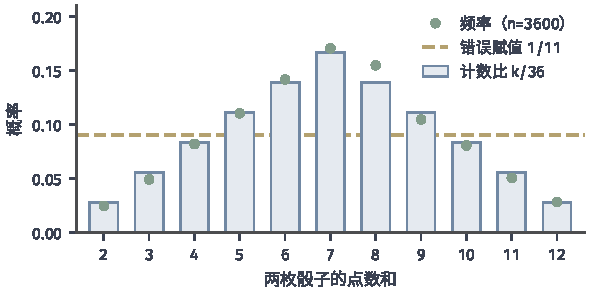
\includegraphics[width=100mm]{figures/07-probability/01-elementary-probability/matplotlib/cprob-dice-sum-frequency/figure.pdf}
  \caption{两枚骰子点数和的概率与频率。浅蓝柱是$36$个有序结果等可能时的概率$k/36$，绿点是$3600$次模拟中的相对频率（随机数种子$7$），黄色虚线是错误地把$11$个点数和看作等可能时的$1/11$。}
  \label{fig:cprob-dice-sum-frequency}
\end{BookInlineFigure}

\paragraph{古典概率与频率}
古典概率和相对频率回答的是不同的问题。古典概率由模型算出，是一个确定的数，不依赖任何实际的投掷；相对频率由观察得到，每做一批试验结果都不同，图~\ref{fig:cprob-coin-frequency}中前几十轮的波动很大。前者是对试验的假设所推出的结论，后者是对试验本身的记录。

两者的联系是：如果模型的等可能假设与试验相符，相对频率在大量重复中会靠近模型给出的概率；如果明显偏离，就说明假设与试验不符，例如一枚灌铅的骰子会让某一面的频率持续偏高。“频率靠近概率”在什么意义下成立，需要先有独立重复试验和随机变量的语言，这一结论在第~\ref{chap:laws-of-large-numbers}章证明。本章只把频率当作检验模型的经验依据，不用它来定义概率。

\paragraph{再看摸球问题}
回到第~\ref{sec:cprob-experiments}节的摸球问题。搅匀后摸球，每个球被第一个摸到的机会相同；摸走一个以后，剩下的四个球被第二个摸到的机会也相同。所以$20$个有序对同样可能，有序记录满足等可能假设。

在有序记录中，“两个都是黑球”有$3\times2=6$个结果，“第一个黑、第二个白”有$3\times2=6$个，“第一个白、第二个黑”有$2\times3=6$个，“两个都是白球”有$2\times1=2$个。于是四个颜色记录的概率分别是
\[
 \frac{6}{20},\quad \frac{6}{20},\quad \frac{6}{20},\quad \frac{2}{20}.
\]
这就是图~\ref{fig:cprob-urn-records}(c)中的数。颜色记录可以作为样本空间，但它的四个点不等可能，不能用计数比；它们的概率要从有序记录算出。第~\ref{sec:cprob-scope}节会专门讨论这种合并带来的问题。
